\documentclass{beamer}
\usepackage{tikz}
\usepackage{amsmath}
\usepackage{pgfplots}
\usepgfplotslibrary{ternary}
\pgfplotsset{compat=1.18}
\usetikzlibrary{arrows.meta, positioning}

\begin{document}

\begin{frame}{Compositional Data Visualization}

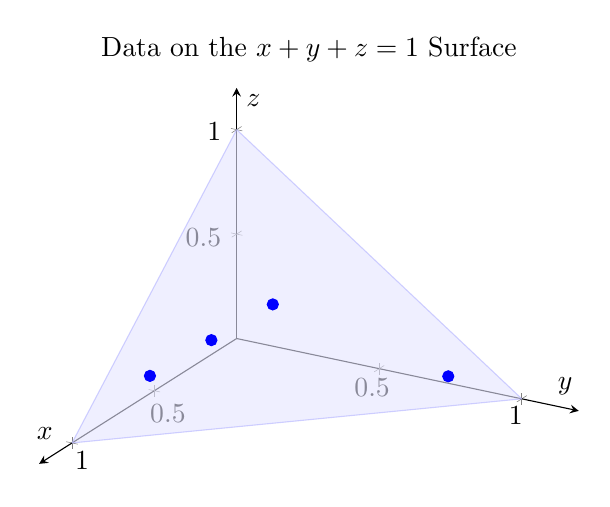
\begin{tikzpicture}
\begin{axis}[
    view={120}{30},
    xlabel=$x$, ylabel=$y$, zlabel=$z$,
    xmin=0, xmax=1.2, ymin=0, ymax=1.2, zmin=0, zmax=1.2,
    axis lines=center,
    title={Data on the $x+y+z=1$ Surface}
]
    % Draw the Simplex Plane (The Surface)
    \addplot3[patch, fill=blue!10, opacity=0.6, faceted color=blue!30] 
        coordinates {(1,0,0) (0,1,0) (0,0,1)};
    
    % Example Data Points on the surface
    \addplot3[only marks, mark=*, blue] coordinates {
        (0.5, 0.2, 0.3)
        (0.1, 0.8, 0.1)
        (0.3, 0.3, 0.4)
        (0.7, 0.1, 0.2)
    };
\end{axis}
\end{tikzpicture}

\end{frame}

\end{document}